\documentclass[journal,12pt,twocolumn]{IEEEtran}

\usepackage{setspace}
\usepackage{gensymb}

\singlespacing


\usepackage[cmex10]{amsmath}

\usepackage{amsthm}

\usepackage{mathrsfs}
\usepackage{txfonts}
\usepackage{stfloats}
\usepackage{bm}
\usepackage{cite}
\usepackage{cases}
\usepackage{subfig}

\usepackage{longtable}
\usepackage{multirow}

\usepackage{enumitem}
\usepackage{mathtools}
\usepackage{steinmetz}
\usepackage{tikz}
\usepackage{circuitikz}
\usepackage{verbatim}
\usepackage{tfrupee}
\usepackage[breaklinks=true]{hyperref}

\usepackage{tkz-euclide}

\usetikzlibrary{calc,math}
\usepackage{listings}
    \usepackage{color}                                            %%
    \usepackage{array}                                            %%
    \usepackage{longtable}                                        %%
    \usepackage{calc}                                             %%
    \usepackage{multirow}                                         %%
    \usepackage{hhline}                                           %%
    \usepackage{ifthen}                                           %%
    \usepackage{lscape}     
\usepackage{multicol}
\usepackage{chngcntr}

\DeclareMathOperator*{\Res}{Res}

\renewcommand\thesection{\arabic{section}}
\renewcommand\thesubsection{\thesection.\arabic{subsection}}
\renewcommand\thesubsubsection{\thesubsection.\arabic{subsubsection}}

\renewcommand\thesectiondis{\arabic{section}}
\renewcommand\thesubsectiondis{\thesectiondis.\arabic{subsection}}
\renewcommand\thesubsubsectiondis{\thesubsectiondis.\arabic{subsubsection}}


\hyphenation{op-tical net-works semi-conduc-tor}
\def\inputGnumericTable{}                                 %%

\lstset{
%language=C,
frame=single, 
breaklines=true,
columns=fullflexible
}
\begin{document}


\newtheorem{theorem}{Theorem}[section]
\newtheorem{problem}{Problem}
\newtheorem{proposition}{Proposition}[section]
\newtheorem{lemma}{Lemma}[section]
\newtheorem{corollary}[theorem]{Corollary}
\newtheorem{example}{Example}[section]
\newtheorem{definition}[problem]{Definition}

\newcommand{\BEQA}{\begin{eqnarray}}
\newcommand{\EEQA}{\end{eqnarray}}
\newcommand{\define}{\stackrel{\triangle}{=}}
\bibliographystyle{IEEEtran}
\providecommand{\mbf}{\mathbf}
\providecommand{\pr}[1]{\ensuremath{\Pr\left(#1\right)}}
\providecommand{\qfunc}[1]{\ensuremath{Q\left(#1\right)}}
\providecommand{\sbrak}[1]{\ensuremath{{}\left[#1\right]}}
\providecommand{\lsbrak}[1]{\ensuremath{{}\left[#1\right.}}
\providecommand{\rsbrak}[1]{\ensuremath{{}\left.#1\right]}}
\providecommand{\brak}[1]{\ensuremath{\left(#1\right)}}
\providecommand{\lbrak}[1]{\ensuremath{\left(#1\right.}}
\providecommand{\rbrak}[1]{\ensuremath{\left.#1\right)}}
\providecommand{\cbrak}[1]{\ensuremath{\left\{#1\right\}}}
\providecommand{\lcbrak}[1]{\ensuremath{\left\{#1\right.}}
\providecommand{\rcbrak}[1]{\ensuremath{\left.#1\right\}}}
\theoremstyle{remark}
\newtheorem{rem}{Remark}
\newcommand{\sgn}{\mathop{\mathrm{sgn}}}
\providecommand{\abs}[1]{\left\vert#1\right\vert}
\providecommand{\res}[1]{\Res\displaylimits_{#1}} 
\providecommand{\norm}[1]{\left\lVert#1\right\rVert}
%\providecommand{\norm}[1]{\lVert#1\rVert}
\providecommand{\mtx}[1]{\mathbf{#1}}
\providecommand{\mean}[1]{E\left[ #1 \right]}
\providecommand{\fourier}{\overset{\mathcal{F}}{ \rightleftharpoons}}
%\providecommand{\hilbert}{\overset{\mathcal{H}}{ \rightleftharpoons}}
\providecommand{\system}{\overset{\mathcal{H}}{ \longleftrightarrow}}
	%\newcommand{\solution}[2]{\textbf{Solution:}{#1}}
\newcommand{\solution}{\noindent \textbf{Solution: }}
\newcommand{\cosec}{\,\text{cosec}\,}
\providecommand{\dec}[2]{\ensuremath{\overset{#1}{\underset{#2}{\gtrless}}}}
\newcommand{\myvec}[1]{\ensuremath{\begin{pmatrix}#1\end{pmatrix}}}
\newcommand{\mydet}[1]{\ensuremath{\begin{vmatrix}#1\end{vmatrix}}}
\numberwithin{equation}{subsection}
\makeatletter
\@addtoreset{figure}{problem}
\makeatother
\let\StandardTheFigure\thefigure
\let\vec\mathbf
\renewcommand{\thefigure}{\theproblem}
\def\putbox#1#2#3{\makebox[0in][l]{\makebox[#1][l]{}\raisebox{\baselineskip}[0in][0in]{\raisebox{#2}[0in][0in]{#3}}}}
     \def\rightbox#1{\makebox[0in][r]{#1}}
     \def\centbox#1{\makebox[0in]{#1}}
     \def\topbox#1{\raisebox{-\baselineskip}[0in][0in]{#1}}
     \def\midbox#1{\raisebox{-0.5\baselineskip}[0in][0in]{#1}}
\vspace{3cm}
\title{Assignment 5}
\author{Gaydhane Vaibhav Digraj \\ Roll No. AI20MTECH11002}
\maketitle
\newpage
\bigskip
\renewcommand{\thefigure}{\theenumi}
\renewcommand{\thetable}{\theenumi}
\begin{abstract}
This document explains the concept of finding the unknown value in an equation such that it is represents two straight lines.
\end{abstract}
%
Download latex-tikz codes from 
%
\begin{lstlisting}
https://github.com/Vaibhav11002/EE5609/tree/master/Assignment_5
\end{lstlisting}
%
\section{Problem}
Find the value of $k$ so that the equation \\$12x^2-10xy+2y^2+11x-5y+k=0$ may represent two straight lines.
\section{Explanation}
Given equation,
\begin{align}
12x^2-10xy+2y^2+11x-5y+k =0 \label{eq:question}
\end{align}
is a second order equation.
The general equation of second degree is given by
\begin{align}
    ax^2+2bxy+cy^2+2dx+2ey+f=0\label{eq:quad_1}\\
    \implies \vec{x}^T\vec{V}\vec{x}+2\vec{u}^T\vec{x}+f=0 \label{eq:quad_2}\\
    \vec{V}=\vec{V}^T=\myvec{a & b \\ b & c} \label{eq:quad_3}\\
    \vec{u}=\myvec{d \\ e} \label{eq:quad_4}
\end{align}
Equation \eqref{eq:quad_2} represents a pair of straight lines if,
\begin{align}
\mydet{\vec{V} & \vec{u}\\\vec{u}^T & f}=0 \label{eq:det_1}
\end{align}
Comparing equation \eqref{eq:question} with \eqref{eq:quad_1}, we can write in the form of \eqref{eq:quad_3} and \eqref{eq:quad_4} as,
\begin{align}
    &\vec{V}=\myvec{12 & -5 \\ -5 & 2} \label{eq:eq1}\\ 
    &\vec{u}=\myvec{\frac{11}{2} \\ \frac{-5}{2}} \label{eq:eq2}\\
    & f=k \label{eq:eq3}
\end{align}
The given equation represent two straight lines, substituting \eqref{eq:eq1}, \eqref{eq:eq2}, \eqref{eq:eq3} in \eqref{eq:det_1} to satisfy the equation.
\begin{align}
    \mydet{12 & -5 & \frac{11}{2} \\ -5 & 2 & \frac{-5}{2}\\\frac{11}{2} & \frac{-5}{2} & k} = 0 \label{eq:solu_1}
\end{align}
Expanding the above determinant along row 3, 
\begin{multline}
    \implies \frac{11}{2}\times(\frac{25}{2}-11) + \frac{5}{2}(-30 + \frac{55}{2}) + k\times(24-25) = 0 \\
\implies \frac{33}{4} + (\frac{-25}{4}) - k = 0 
\end{multline}
\begin{align}
    \implies \boxed{k=2} \label{eq:result}
\end{align}
\section{Solution}
For $k = 2$ the given equation will represent two straight lines.
\begin{align}
12x^2-10xy+2y^2+11x-5y+2 = 0 \label{eq:op1}
\end{align}
From \eqref{eq:op1} we get, 
\begin{align}
    f = 2 \label{eq:f_value} \\
    \det(V) = \mydet{12 & -5 \\ -5 & 2} = -1 < 0 
\end{align}
Since $\det(V)<0$ we can say that two intersecting lines are obtained.

\renewcommand{\thefigure}{\arabic{figure}}
\begin{figure}[h!]
	\centering
	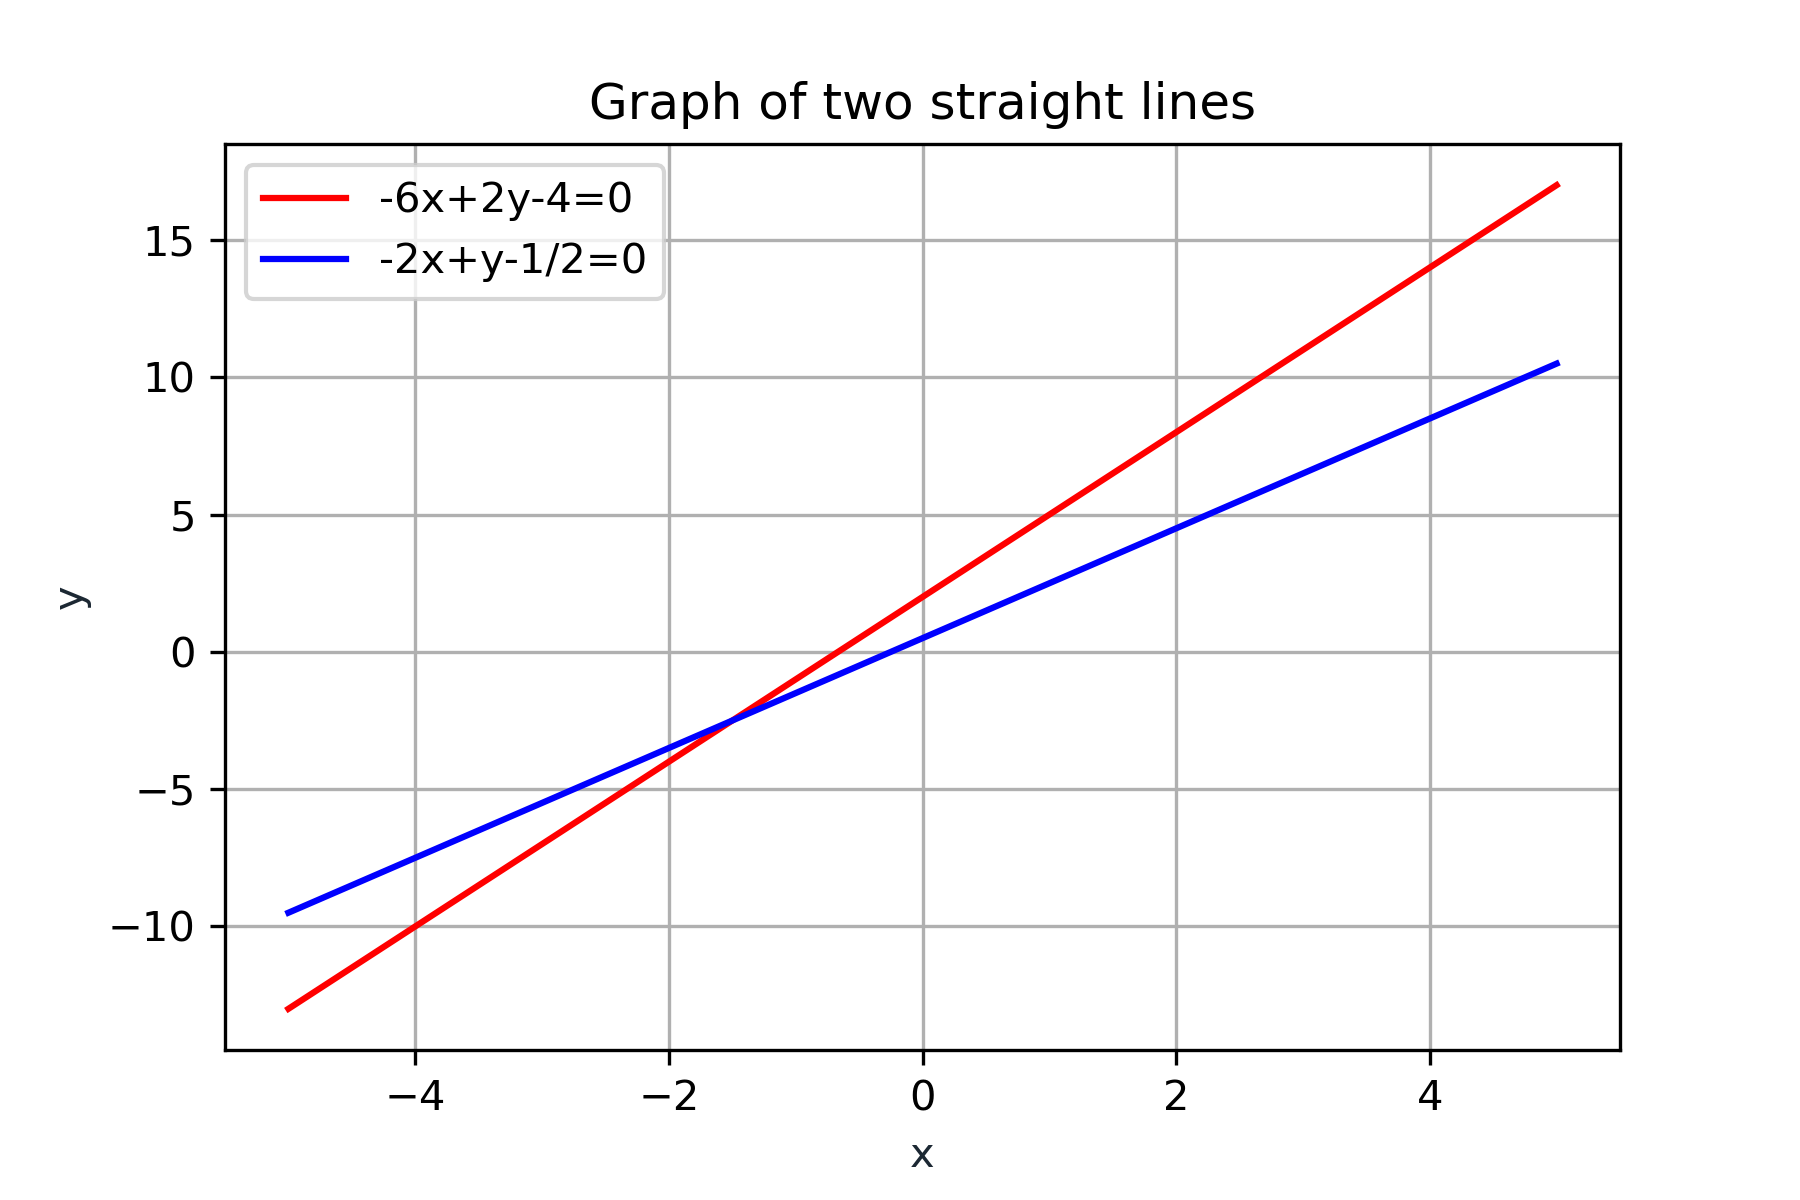
\includegraphics[width=\columnwidth]{straightlines.png}
	\caption{Plot of Straight lines}
	\label{fig_1}
\end{figure}

The pair of straight lines in vector form is given by, 
\begin{align}
    \vec{n_1}^T\vec{x}&=c_1\label{m1}\\
    \vec{n_2}^T\vec{x}&=c_2\label{m2}
\end{align}
Equating their product with \eqref{eq:quad_2}, 
\begin{align}
    (\vec{n_1}^T\vec{x}-c_1)(\vec{n_2}^T\vec{x}-c_2)
    = \vec{x}^T\vec{V}\vec{x}+2\vec{u}^T\vec{x}+f=0
\end{align}
\begin{align}
\vec{n_1}*\vec{n_2}=\{12,-10,2\}\label{conv}\\
c_2\vec{n_1}+c_1\vec{n_2} = -2\vec{u} =  -2\myvec{\frac{11}{2}\\ \frac{-5}{2}} \label{eqc1c2}\\
c_1c_2 = f = 2
\end{align}
The slopes of the lines are given by the roots of the polynomial 
\begin{align}
    &cm^2+2bm+a=0\label{e}\\
    \implies m_i&=\frac{-b\pm{\sqrt{-\det(V)}}}{c}\\
    \vec{n_i}&=k\myvec{-m_i\\1}
\end{align}
Substituting the given data in above equations \eqref{e} we get,
\begin{align}
    &2m^2 -10m + 12 = 0\\
    &\implies m_i = \frac{-(-5)\pm{\sqrt{-(-1)}}}{2}\label{m}
\end{align}
Solving equation \eqref{m} we get ,
\begin{align}
    m_1&= 3 \\
    m_2&= 2 \\
    \vec{n_1}&=k_1\myvec{-3 \\ 1}\label{n1}\\
    \vec{n_2}&=k_2\myvec{-2 \\ 1}\label{n2}
\end{align}
Substituting equations \eqref{n1}, \eqref{n2} in equation \eqref{conv} 
\begin{align}
    k_1k_2 &= 2
\end{align}
The possible combinations of ($k_1,k_2$) are (1,2), (2,1), (-1,-2), (-2,-1). 
Let's assume $k_1=2$, $k_2=1$, we get 
\begin{align}
    \vec{n_1}&=\myvec{-6 \\ 2}\label{n11}\\
    \vec{n_2}&=\myvec{-2 \\ 1}\label{n22}
\end{align}

We have:
\begin{align}
\vec{n_1}\ast \vec{n_2} = \myvec{a\\2b\\c} \label{eq:conv1}
\end{align}

Convolution of $\vec{n_1}$ and $\vec{n_2}$ can be done by converting  $\vec{n_1}$ into a teoplitz matrix and multiplying with $\vec{n_2}$\\
From equation \eqref{n11} and \eqref{n22}. 
\begin{align}
    \vec{n_1}=\myvec{-6 & 0 \\ 2 & -6 \\ 0 & 2}
    \vec{n_2}=\myvec{-2 \\ 1} \label{eq:conv2}\\
    \implies\myvec{-6 & 0 \\ 2 & -6 \\ 0 & 2}\myvec{-2 \\ 1} = \myvec{12 \\ -10 \\ 2} = \myvec{a\\2b\\c}\label{eq:conv3}
\end{align}

$c_1$ and $c_2$ can be obtained as, 
\begin{align}
    \myvec{\vec{n_1} & \vec{n_2}}\myvec{c_2\\c_1} & =-2\myvec{\frac{11}{2}\\\frac{-5}{2}} \\
    \myvec{-6 & -2 \\2 & 1}\myvec{c_2\\c_1} &= \myvec{-11 \\ 5} \label{eq:aug}
\end{align}
Converting \eqref{eq:aug} to augmented matrix and solving using row reduction, 
\begin{align}
    \myvec{-6 & -2 & -11 \\ 2 & 1 & 5} \xleftrightarrow[]{R1 \xleftarrow{} \frac{R1}{-6}} \myvec{1 & \frac{1}{3} & \frac{11}{6} \\ 2 & 1 & 5} \\
    \myvec{1 & \frac{1}{3} & \frac{11}{6} \\ 2 & 1 & 5}\xleftrightarrow[]{R2 \xleftarrow{} R2-2R1 } \myvec{1 & \frac{1}{3} & \frac{11}{6} \\ 0 & \frac{1}{3} & \frac{4}{3}} \\ 
    \myvec{1 & \frac{1}{3} & \frac{11}{6} \\ 0 & \frac{1}{3} & \frac{4}{3}}
    \xleftrightarrow[]{R1 \xleftarrow{} R1-R2} \myvec{1 & 0 & \frac{1}{2} \\ 0 & \frac{1}{3} & \frac{4}{3}} \\
    \myvec{1 & 0 & \frac{1}{2} \\ 0 & \frac{1}{3} & \frac{4}{3}}
    \xleftrightarrow[]{R2 \xleftarrow{} 3R2} \myvec{1 & 0 & \frac{1}{2} \\ 0 & 1 & 4}
\end{align}
Thus we get, 
\begin{align}
    c_1 &= 4\\
    c_2 &= \frac{1}{2}
\end{align}

Equations \eqref{m1}, \eqref{m2} can be modified as, 
\begin{align}
    \myvec{-6 & 2}\vec{x} &= 4\\
    \myvec{-2 & 1}\vec{x} &= \frac{1}{2}
\end{align}
\end{document}
